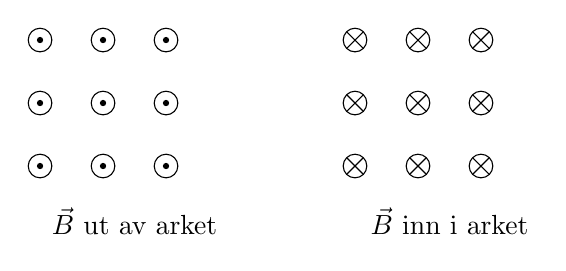
\begin{tikzpicture}
\foreach \x in {0,0.8,...,2.4} \foreach \y in {0,0.8,...,2.4} { \draw (\x,\y) circle (0.15); \fill (\x,\y) circle (0.04); }
\node[below] at (1.2,-0.4) {$\vec B$ ut av arket};
\begin{scope}[xshift=4cm]
\foreach \x in {0,0.8,...,2.4} \foreach \y in {0,0.8,...,2.4} { \draw (\x,\y) circle (0.15); \draw (\x-0.1,\y-0.1) -- (\x+0.1,\y+0.1); \draw (\x-0.1,\y+0.1) -- (\x+0.1,\y-0.1); }
\node[below] at (1.2,-0.4) {$\vec B$ inn i arket};
\end{scope}
\end{tikzpicture}
